
\section{Халькогены. Отличительные свойства кислорода, озон. Химические свойства простых веществ халькогенов. Водородные соединения халькогенов, их оксиды и кислородные кислоты.}

\textbf{Халькогены} --- элементы главной подгруппы 6(16) группы: неметаллы --- кислород \ce{O}, сера \ce{S}, селен \ce{Se}; мтеаллоид теллур \ce{Te} и радиоактивный металл полоний \ce{Po}.

Электронная конфигурация внешнего уровня --- $ns^2np^4$.

Низшая степень окисления --- -2.

Все элементы (кроме кислорода) образуют соединения, в которых степень окисления равна +4, +6.

Главные герои этого билета --- кислород и сера.

\subsection{Кислород}

Кислород образует два простых вещества --- молекулярный кислород \ce{O2} и озон \ce{O3}.

Кислород парамагнитен, а озон даимагнитен.\\

\textbf{Кислород} --- сильный окислитель, реагирует с большинством металлов, образуя основные оксиды, и с неметалллами, образуя кислотные оксиды:

\begin{equation*}
\ce{2Cu + O2 -> 2CuO}
\end{equation*}
\begin{equation*}
\ce{4P + 5O2 -> 2P2O5}
\end{equation*}
\begin{equation*}
\ce{S + O2 -> SO2}
\end{equation*}

Реагирует с многими соединениями: сульфидами, гидридами, низшими оксидами:

\begin{equation*}
\ce{4NH3 + 3O2 -> 2N2 + 6H2O}
\end{equation*}
\begin{equation*}
\ce{2CuS + 3O2 -> 2CuO + 2SO2}
\end{equation*}
\begin{equation*}
\ce{2NO + O2 -> 2NO2}
\end{equation*}

Несмотря на высокую химическую активность, кислород не реагирует ни с кислотами, ни с щелочами.

Кислород как донор электронов ообразует комплексы с железосодержащими белками, например, гемоглобином \ce{Hb}:
\begin{equation*}
\ce{Hb + O2 -> Hb \cdot O2}
\end{equation*}
Молекула гемоглобина может связывать до 4 молекул кислорода.

Получается в лаборатории разложением некоторых солей кислородсодержащих кислот, оксидов и пероксидов:

\begin{equation*}
\ce{2KMnO4 ->T[\text{t}] K2MnO4 + MnO2 + O2 ^}
\end{equation*}
\begin{equation*}
\ce{2KClO3 ->T[\text{t}] 2KCl + 3O2 ^}
\end{equation*}
\begin{equation*}
\ce{2H2O2 ->T[\text{катализатор}] 2H2O + O2 ^}
\end{equation*}

\textbf{Озон} --- сильнейший окислитель, очень ядовит.

Качественная реакция: взаимодействие с раствором йодида калия (посинение раствора, содержащего крахмал, например):

\begin{equation*}
\ce{2KI + O3 + H2O -> I2 + 2KOH + O2}
\end{equation*}

Окисление сульфида свинца в сульфат (цвет сменяется с черного на белый):

\begin{equation*}
\ce{3PbS + 4O3 -> 3PbSO4}
\end{equation*}

Озон окисляет большинство металлов (кроме благородных) и многие неметаллы до оксидов, соответствующих их высшей степени окисления:

\begin{equation*}
\ce{S + O3 -> SO3}
\end{equation*}

Образование серной кислоты:

\begin{equation*}
\ce{O3 + S + H2O -> H2SO4}
\end{equation*}

\subsection{Сера}

В лаборатории серу получают путем неполного окисления сероводорода:

\begin{equation*}
\ce{2H2S + O2 -> 2S + 2H2O}\ \text{(недостаток \ce{O2})}
\end{equation*}

Сера --- довольно активный неметалл. Реагирует при комнатной температуре со фтором, хлором и концентрированными кислотами-окислителями:

\begin{equation*}
\ce{S + 3F2 -> SF6}
\end{equation*}

\begin{equation*}
\ce{S + 2H2SO4}\text{(конц.) } \ce{-> 3SO2 ^ + 2H2O}
\end{equation*}

На воздухе сера горит, образуя \ce{SO2}. Во всех указанных реакциях сера --- восстановитель.

Окислительные свойства проявляет в реакциях с водородом и металлами:

\begin{equation*}
\ce{H2 + S -> H2S}
\end{equation*}
\begin{equation*}
\ce{Fe + S -> FeS}
\end{equation*}
\begin{equation*}
\ce{Hg + S -> HgS}
\end{equation*}

Последняя реакция описывает возможность удаления разлитой ртути.

Сера при нагревании растворяется в щелочах, при этом происходит реакция диспропорционирования:

\begin{equation*}
\ce{3S + 6NaOH -> Na2SO3 + 2Na2S + 3H2O}
\end{equation*}

\subsection{Водородные соединения}
\subsubsection{Пероксид водорода}
\begin{figure}[H]
	\centering
	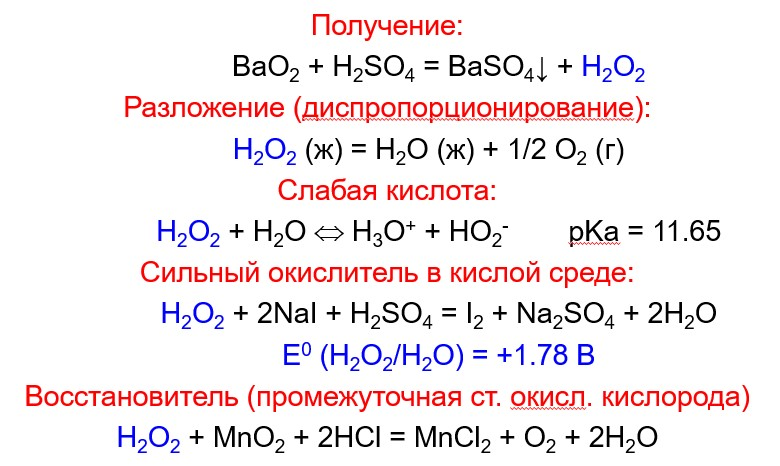
\includegraphics[width=0.7\linewidth]{Pictures/Peroxide.jpg}
	\caption{Свойства пероксида водорода.}
\end{figure}
\subsubsection{Сероводород}
Получение чистого сероводорода:

\begin{equation*}
\ce{Al2S3_{solid} + 6H2O_{liquid} -> 2Al(OH)3 v + 3H2S ^}
\end{equation*}

Так как сера в сероводороде имеет низшую степень окусления, он проявляет сильные восстановительные свойства. Например, легко окисляется галогенами:

\begin{equation*}
\ce{H2S + Br2 -> S v + 2 HBr}
\end{equation*}

Раствор сероводорода в воде - слабая двухосновная кислота, тоже типичный восстановитель:
\begin{equation*}
\ce{2H2S + SO2 -> 3S v + 2H2O}
\end{equation*}

Сероводородная кислота образует два ряда солей: средние --- сульфиды, кислые --- гидросульфиды.
\subsubsection{Сульфиды}

Растворимые в воде сульфиды сильно гидролизованы:

\begin{equation*}
\ce{Na2S + H2O <--> NaHS + NaOH}
\end{equation*}

Многие сульфиды растворимы в сильных кислотах:
\begin{equation*}
\ce{FeS + 2HCl -> FeCl2 + H2S ^}
\end{equation*}

Сульфиды тяжелых металлов нерастворимы в кислотах (\ce{CuS}, \ce{PbS}, \ce{HgS}, \ce{Ag2S}).

\subsection{Оксиды и кислородные кислоты}
\subsubsection{Диоксид серы. Сернистая кислота.}
Сера в степени окисленя +4.
Диоксид серы образуется при сжигании сульфидов, сероводорода и восстановлении серной кислоты:
\begin{equation*}
\ce{2CuS + 3O2 -> 2CuO + 2SO2}
\end{equation*}

Легко окисляется до \ce{S^+6}:
\begin{equation*}
\ce{SO2 + Br2 + H2O -> H2SO4 + 2HBr}
\end{equation*}

Раствор оксида в воде - двухосновная сернистая кислота. Её соли -- сульфиты -- восстановители:

\begin{equation*}
\ce{SO2 + 2NaOH -> Na2SO3 + H2O}
\end{equation*}

Слабый окислитель (восстанавливается сильным восстановителем):
\begin{equation*}
\ce{H2SO3 + 2H2S -> 3S + 2H2O}
\end{equation*}

\subsubsection{Серный ангидрид. Серная кислота.}
Серный ангидрид образуется при каталитическом окислении диоксида:

\begin{equation*}
\ce{2SO2 + O2 -> 2SO3}
\end{equation*}

Очень гигроскопичен, раствор ангидрида в серной кислоте --- олеум:

\begin{equation*}
\ce{SO3 + H2O -> H2SO4}
\end{equation*}

Сильный окислитель:

\begin{equation*}
\ce{5SO3 + 2P -> P2O5 + 5SO2}
\end{equation*}

\textbf{Серная кислота} --- сильная двухосновная кислота. Окислитель при больших концентрациях:

\begin{equation*}
\ce{Cu + 2H2SO4}\text{(конц.)} \ce{-> CuSO4 + SO2 + 2H2O}
\end{equation*}
\begin{equation*}
\ce{2P + 5H2SO4}\text{(конц.)} \ce{-> 2H3PO4 + 5SO2 + 2H2O}
\end{equation*}

Сильное водоотнимающее средство:
\begin{equation*}
\ce{C12H22O11 + H2SO4 -> 12C + 11H2O + Q }
\end{equation*}

\subsubsection{Бинарные соединения кислорода}
\begin{figure}[H]
	\centering
	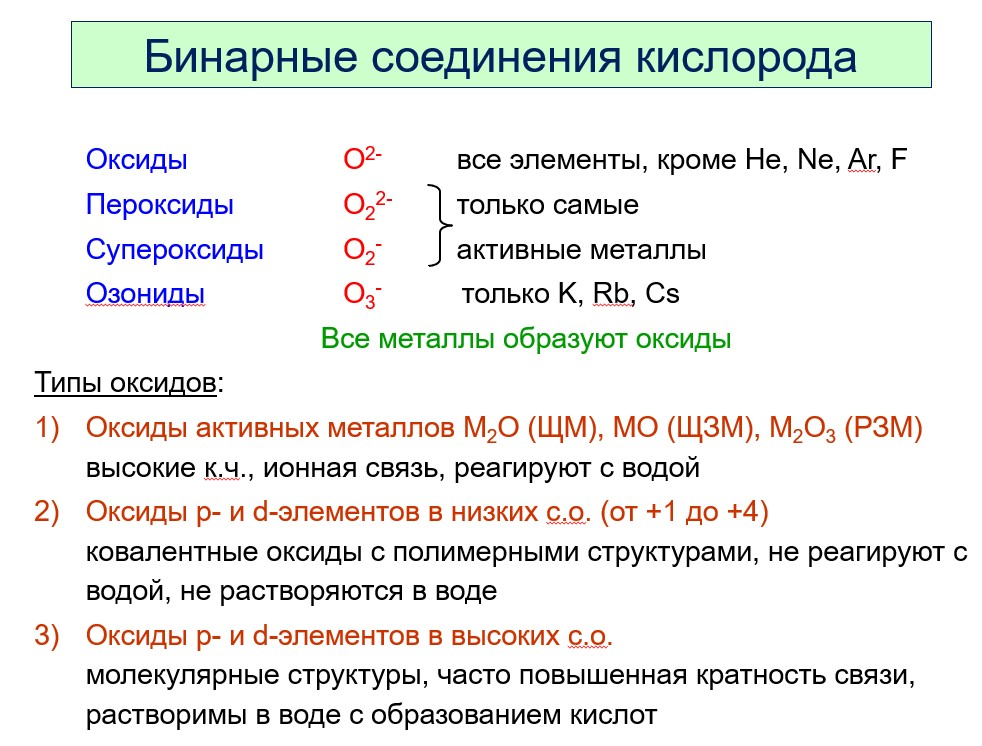
\includegraphics[width=0.7\linewidth]{Pictures/Bin.jpg}
	\caption{Бинарные соединения кислорода.}
\end{figure}

\subsubsection{Качественные реакции}
\begin{figure}[H]
	\centering
	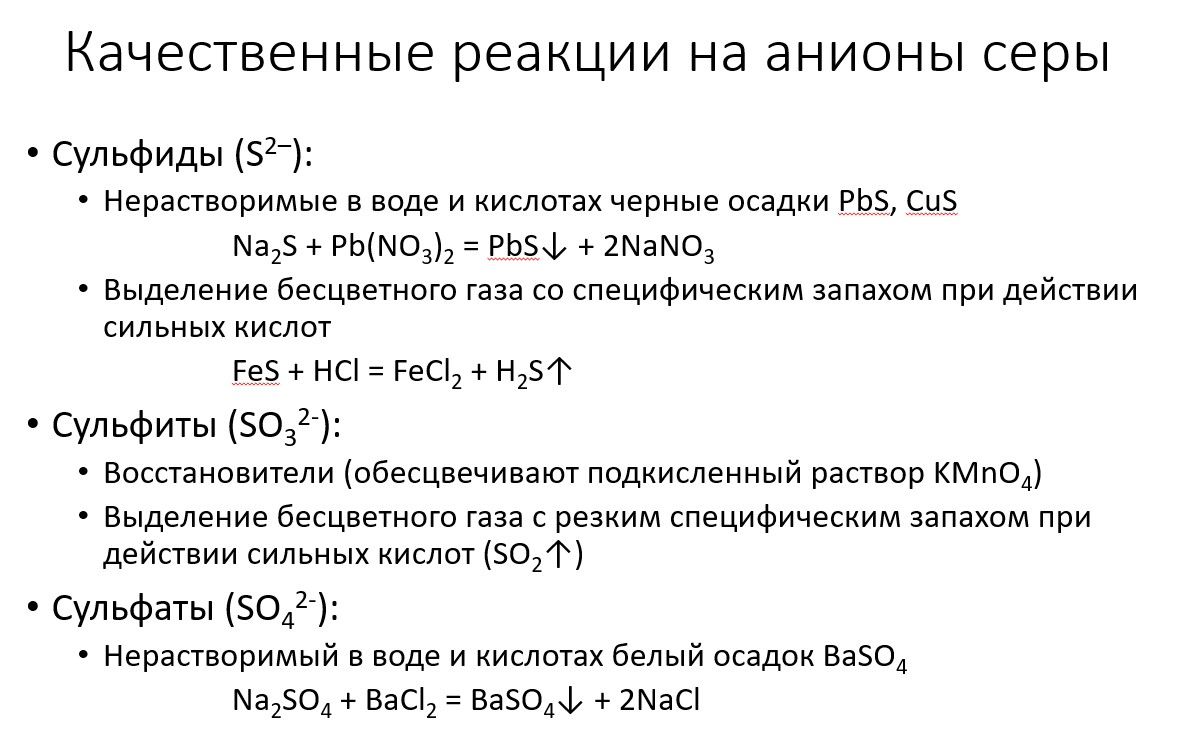
\includegraphics[width=0.7\linewidth]{Pictures/Kach.jpg}
	\caption{Качественные реакции.}
\end{figure}

\subsection{Селен и Теллур}
\begin{figure}[H]
	\centering
	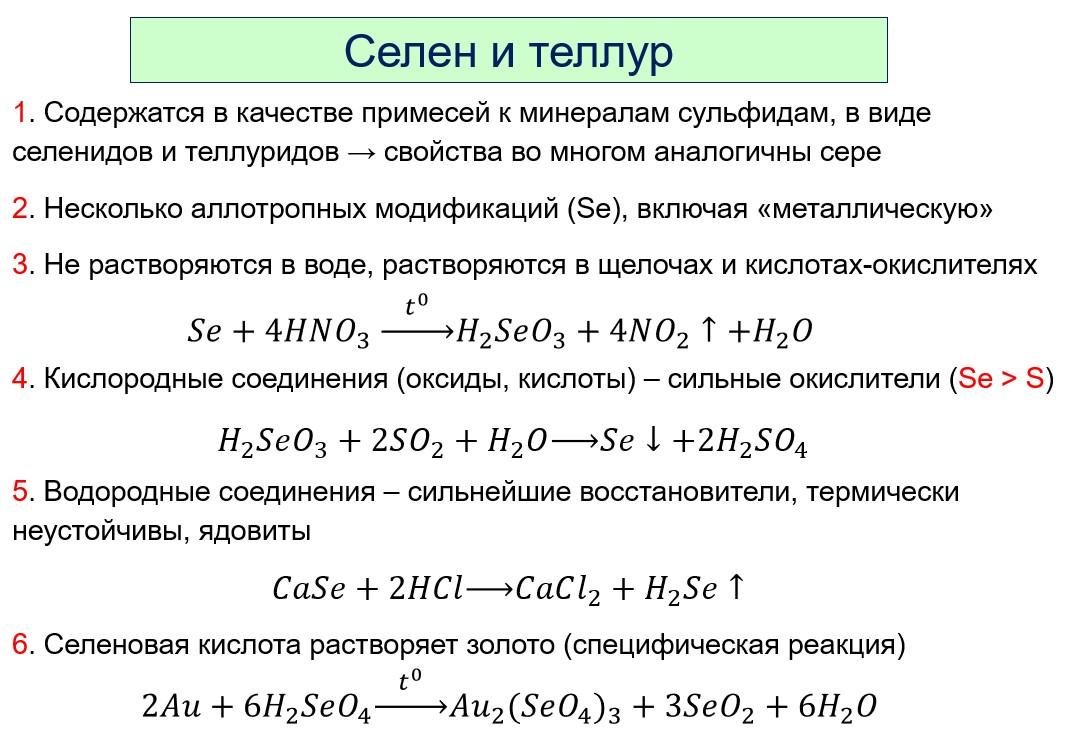
\includegraphics[width=0.7\linewidth]{Pictures/Se.jpg}
	\caption{Селен и Теллур.}
\end{figure}
